\documentclass[10pt,landscape]{report}
\usepackage[usenames,dvipsnames,svgnames,table]{xcolor}
\usepackage{tikz}
\usepackage{graphicx}
\usepackage{wallpaper}
\usepackage[landscape]{geometry}
\newgeometry{margin=1cm}
\usetikzlibrary{shapes,arrows,decorations.pathmorphing,shadows.blur,graphs,chains}
\tikzstyle{b1}=[fill=red,draw,decorate,decoration={bent,aspect=.2},
minimum height=2cm, text width=3cm, text centered, blur shadow={shadow blur steps=5},font=\small, text=white]
\tikzstyle{box1}=[rectangle, draw=black, rounded corners, fill=blue!80, drop shadow,
        text centered, anchor=north, text=white, text width=3cm, font=\small]
\tikzstyle{point}=[rectangle, rounded corners=2pt, text width=3cm, minimum height=2cm, draw=black, fill=black!80, drop shadow, text=white, text centered, font=\small]
\tikzstyle{box2}=[rectangle, draw=black, rounded corners, fill=blue!50!black!50, drop shadow,
        text centered, anchor=north, text=white, text width=3cm, font=\small]
\tikzstyle{point2}=[rectangle, rounded corners=2pt, text width=6cm, minimum height=1cm, draw=black, fill=black!80, drop shadow, text=white, text centered, font=\small]
\usepackage{eso-pic}
\newcommand\BackgroundPic{
\put(0,0){
\parbox[b][\paperheight]{\paperwidth}{%
\vfill
\centering
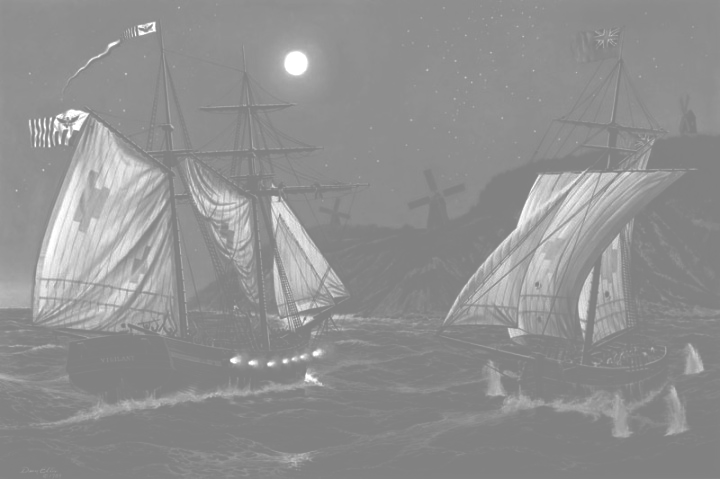
\includegraphics[width=\paperwidth,height=\paperheight,
keepaspectratio]{war.png}%
\vfill
}}}
\begin{document}
\AddToShipoutPicture{\BackgroundPic}
\begin{tikzpicture}[start chain=1 going right, start chain=2 going right,start chain=3 going right,
			node distance=5mm]
\node [box1, on chain=1]{1787};
\node [box1, on chain=1]{1798};
\node [box1, on chain=1]{1799};
\node [box1, on chain=1]{1812};
\node [box1, on chain=1]{1846};
\node [box1, on chain=1]{1861};
\node [box1, on chain=1]{1865};
\node [b1, on chain=2]at (0, -2){U.S Constitution signed on September 17th};
\node [b1, on chain=2] {Quasi-War with France authorized by Congress on May 28th};
\node [b1, on chain=2] {Quasi-War};
\node [b1, on chain=2] {War of 1812};
\node [b1, on chain=2] {Mexican-American War};
\node [b1, on chain=2] {Civil War};
\node [b1, on chain=2] {Civil War};
\node (flag1)[drop shadow={shadow scale=0.94, top color=gray, opacity=0.5
}] at (5.6,-8){
\includegraphics[scale=0.1]{Flag_of_France.png}};
\node (flag2)[drop shadow={shadow scale=0.94, top color=gray, opacity=0.5
}] at (11.3,-16.5){
\includegraphics[scale=0.089]{Flag_of_the_United_Kingdom.png}};
\node (flag2)[drop shadow={shadow scale=0.94, top color=gray, opacity=0.5
}] at (15,-11){
\includegraphics[scale=0.07]{Flag_of_Mexico.png}};
\node (flag2)[drop shadow={shadow scale=0.94, top color=gray, opacity=0.5
}] at (22.5,-5){
\includegraphics[scale=0.1]{Confederate_Rebel_Flag.png}};
\node (flag2)[drop shadow={shadow scale=0.94, top color=gray, opacity=0.5
}] at (22.5,-8){
\includegraphics[scale=0.089]{Flag_of_the_United_States.png}};

\node [point, on chain=3]at (3.8,-5) {The cutter Pickering captured 10 prizes, one of which carried 44 guns
and 200 men, three times her own force.};
\node [point, on chain=3]{The Eagle, recaptured the American vessels
Nancy and Mehitable in a memorable fight in 1799 with the French
privateer, Revenge.};
\node [point, on chain=3]{The cutter Jefferson
captured the first prize of this war.};
\node [point, on chain=going below] {One of the most hotly contested battles was between the cutter
Surveyor and the British frigate Narcissis. The Surveyor was
eventually captured, but the British captain praised the gallantry of the
American crew.
};
\node [point, on chain=going below]{One of the most dramatic engagements was the defense of the cutter
Eagle against the attack of the British brig Dispatch and an
accompanying sloop.
};
\node [point, on chain=3]at (12.9, -6.5) {After combat skirmishes with American and Mexican troops over the
Texas southwestern boundary, Congress declared war with Mexico on
May 13, 1846. Mexico’s declaration of war with the U.S. occurred on
May 23rd.
};
\node [point, on chain=3]{The cutter
Harriet Lane took part in the expedition to Fort Sumter in 1861 to patrol
the coast for commerce raiders and provide fire support for troops ashore.
The Harriet Lane is credited with firing the first naval shots of the Civil
War.
};

\end{tikzpicture}
\clearpage
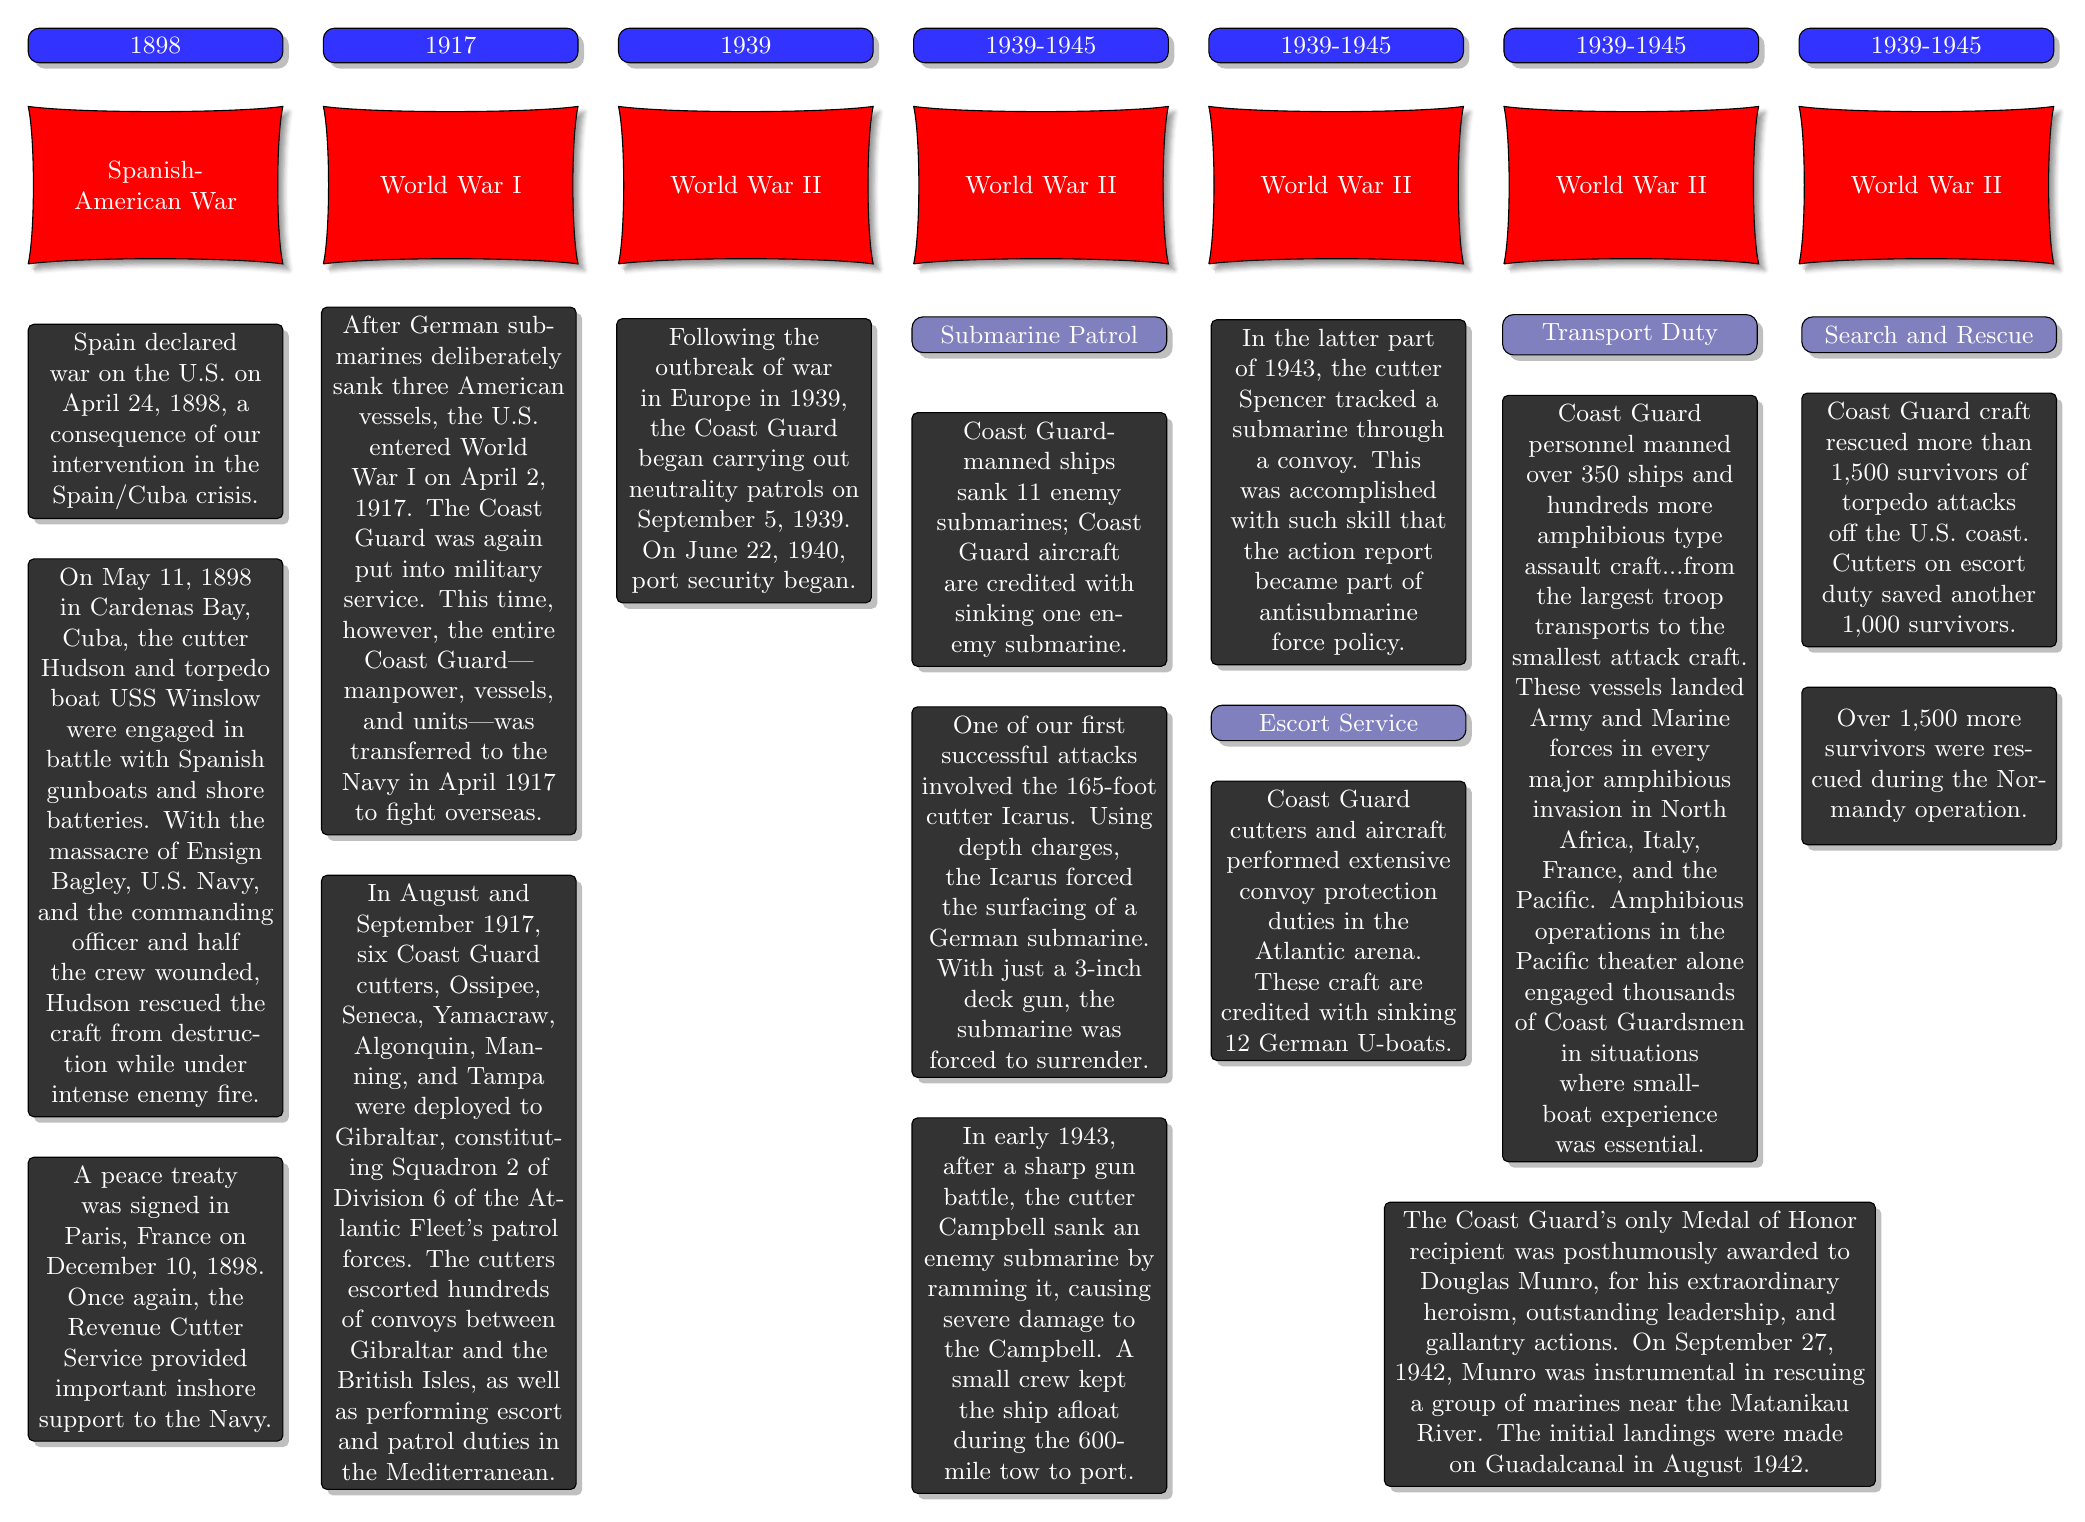
\begin{tikzpicture}[start chain=4 going right, start chain=5 going right, start chain=6 going right, node distance=5mm]
\node [box1, on chain=4]{1898};
\node [b1, on chain=5]at (0,-2) {Spanish-American War};
\node [point, on chain=6] at (0,-5){Spain declared war on the U.S. on April 24, 1898, a consequence of our
intervention in the Spain/Cuba crisis.
};
\node [point, on chain=going below]{On May 11, 1898 in Cardenas Bay, Cuba, the cutter Hudson and torpedo
boat USS Winslow were engaged in battle with Spanish gunboats and
shore batteries. With the massacre of Ensign Bagley, U.S. Navy, and the
commanding officer and half the crew wounded, Hudson rescued the craft
from destruction while under intense enemy fire.
};
\node [point, on chain=going below]{A peace treaty was signed in Paris, France on December 10, 1898. Once
again, the Revenue Cutter Service provided important inshore support to
the Navy.
};
\node [box1, on chain=4]{1917};
\node [box1, on chain=4]{1939};
\node [box1, on chain=4]{1939-1945};
\node [box1, on chain=4]{1939-1945};
\node [box1, on chain=4]{1939-1945};
\node [box1, on chain=4]{1939-1945};
\node [b1, on chain=5]{World War I};
\node [b1, on chain=5]{World War II};
\node [b1, on chain=5]{World War II};
\node [b1, on chain=5]{World War II};
\node [b1, on chain=5]{World War II};
\node [b1, on chain=5]{World War II};
\node [point, on chain=6] at (1.6,-6.9) {After German submarines deliberately sank three American vessels, the
U.S. entered World War I on April 2, 1917. The Coast Guard was again
put into military service. This time, however, the entire Coast Guard—
manpower, vessels, and units—was transferred to the Navy in April 1917
to fight overseas.
};
\node [point, on chain=going below]{In August and September 1917, six Coast Guard cutters, Ossipee, Seneca,
Yamacraw, Algonquin, Manning, and Tampa were deployed to Gibraltar,
constituting Squadron 2 of Division 6 of the Atlantic Fleet’s patrol forces.
The cutters escorted hundreds of convoys between Gibraltar and the
British Isles, as well as performing escort and patrol duties in the
Mediterranean.
};
\node [point, on chain=6] at (5.35,-5.5) {Following the outbreak of war in Europe in 1939, the Coast Guard began
carrying out neutrality patrols on September 5, 1939. On June 22, 1940,
port security began.
};
\node [box2, on chain=6] at (9.1, -3.9) {Submarine Patrol};
\node [point, on chain=6] at (9.1, -6.5) {Coast Guard-manned ships sank 11 enemy submarines; Coast Guard
aircraft are credited with sinking one enemy submarine.};
\node [point, on chain=going below]{One of our first successful attacks involved the 165-foot cutter
Icarus. Using depth charges, the Icarus forced the surfacing of a
German submarine. With just a 3-inch deck gun, the submarine
was forced to surrender.
};
\node [point, on chain=going below]{In early 1943, after a sharp gun battle, the cutter Campbell sank an
enemy submarine by ramming it, causing severe damage to the
Campbell. A small crew kept the ship afloat during the 600-mile
tow to port.};
\node [point, on chain=6] at (12.9, -5.9) {In the latter part of 1943, the cutter Spencer tracked a submarine
through a convoy. This was accomplished with such skill that the
action report became part of antisubmarine force policy.
};
\node [box2, on chain=going below]{Escort Service};
\node [point, on chain=going below]{Coast Guard cutters and aircraft performed extensive convoy protection
duties in the Atlantic arena. These craft are credited with sinking 12
German U-boats.
};
\node [box2, on chain=6]at (16.6,-3.9){Transport Duty};
\node [point, on chain=going below]{Coast Guard personnel manned over 350 ships and hundreds more
amphibious type assault craft...from the largest troop transports to the
smallest attack craft. These vessels landed Army and Marine forces in
every major amphibious invasion in North Africa, Italy, France, and the
Pacific. Amphibious operations in the Pacific theater alone engaged
thousands of Coast Guardsmen in situations where small-boat experience
was essential.
};
\node [point2, on chain=going below]{The Coast Guard’s only Medal of Honor recipient was posthumously
awarded to Douglas Munro, for his extraordinary heroism, outstanding
leadership, and gallantry actions. On September 27, 1942, Munro was
instrumental in rescuing a group of marines near the Matanikau River.
The initial landings were made on Guadalcanal in August 1942.
};
\node [box2, on chain=6]at(20.4,-3.9){Search and Rescue};
\node [point, on chain=going below]{Coast Guard craft rescued more than 1,500 survivors of torpedo attacks off the U.S. coast. Cutters on escort duty saved another 1,000 survivors.};
\node [point, on chain=going below]{Over 1,500 more survivors were rescued during the Normandy operation.};
\end{tikzpicture}

\clearpage
\begin{tikzpicture}[start chain=7 going right, start chain=8 going right, start chain=9 going right, node distance=5mm]

\node [box1, on chain=7]{1939-1945};
\node [box1, on chain=7]{1946};
\node [box1, on chain=7]{1946};
\node [box1, on chain=7]{1950};
\node [box1, on chain=7]{1965-1970};
\node [box1, on chain=7]{1990-1991};
\node [box1, on chain=7]{2001-Current};
\node [b1, on chain=8] at (0,-2){World War II};
\node [b1, on chain=8] {Return to the Treasury Department};
\node [b1, on chain=8] {Prior to Korean War};
\node [b1, on chain=8] {Korean War};
\node [b1, on chain=8] {Vietnam Conflict};
\node [b1, on chain=8] {Desert Shield/Storm};
\node [b1, on chain=8] {War on Terrorism};
\node [box2, on chain=going below]at (0,-3.5){Water and Shore
Patrol};
\node [point, on chain=going below]{Coast Guard coastal picket vessels patrolled along the 50-fathom curve, where enemy submarines concentrated early in the war. As a major
participant in the U.S. anti-sabotage effort, on-shore duty had armed Coast
Guardsmen patrolling beaches and docks};
\node [box2, on chain=going below]{“Rear” Support
Services};
\node [point, on chain=going below]{The Coast Guard also contributed to the war effort in other less publicized areas. These activities included, Providing port security, Supervising the movement of dangerous cargoes, Controlling merchant vessel traffic, Maintaining aids to navigation, Breaking ice to allow ship passage};
\node [point, on chain=9] at (1.6,-4.7) {The Coast Guard returned under the jurisdiction of the Treasury Department on January 1, 1946.};
\node (flag6)at (3.7, -7.3)[drop shadow={shadow scale=.94, top color=gray, opacity=0.5
}] {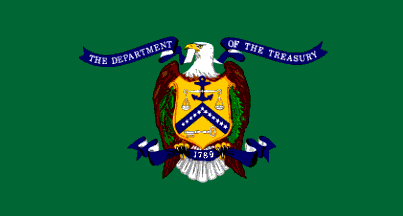
\includegraphics[scale=0.3]{Treasury.png}};
\node [point, on chain=9] at (5.4,-7.2){In 1946, a Coast Guard
team was sent to Seoul, Korea to organize, supervise, and train a South
Korean Coast Guard. They succeeded in establishing a shipyard, supply
and communications systems, and training facilities. The team also
arranged for the transfer of 19 ships from the Japanese and American
navies.};
\node [point, on chain=9]at (9.1, -7.6) {When “war” broke out, the Coast Guard’s role was marginal, primarily
one of support. Its principal contributions consisted of improving
communications and meteorological services, as well as assuring port
security and proper ammunition handling. Coast Guardsmen manned a
number of Navy destroyer escorts, performing a variety of missions in the
Western Pacific.};
\node (flag6)at (9.1, -13.4) [drop shadow={shadow scale=.94, top color=gray, opacity=0.5
}] {
\includegraphics[scale=0.3]{Flag_of_North_Korea.png}};
\node [point, on chain=9]at (12.9,-7.8) {The Coast Guard was also an effective force in the Vietnam Conflict, performing duties uniquely suited to its specialized skills.
Shallow-draft warships and operating expertise in coastal waters were
needed for the interdiction of trawlers being used by North Vietnam for
infiltration and resupply activities. This operation was named “Market
Time,” with the Coast Guard having a major role.};
\node (flag6)at (15, -13.5) [drop shadow={shadow scale=.94, top color=gray, opacity=0.5
}] {
\includegraphics[scale=0.5]{Flag_of_Vietnam.png}};
\node [point, on chain=9]at (16.65, -7.6) {The mission of Operation Desert Shield was to defend Saudi Arabia.
After invading Kuwait, Iraqi troops had begun to mass along the Saudi
border, breaching it at some points. This suggested that Hussein’s forces
may continue south into Saudi Arabia’s oil fields.
When it was obvious that Saddam would not withdraw, Desert Shield
became Desert Storm on January 17, 1991.};
\node (flag6)at (18.75, -13.5) [drop shadow={shadow scale=.94, top color=gray, opacity=0.5
}] {
\includegraphics[scale=0.5]{Iraq.png}};
\node [box2, on chain=9] at (20.35,-4.1) {Operation Liberty Shield In March 2002};
\node [point, on chain=going below] {As part of this operation,
the Coast Guard increased its patrols by 50 percent and placed armed
boarding officers on every high-interest vessel arriving or departing
from American ports. By the end of 2003, the USCG had conducted
over 3,000 air and sea patrols. Over 3,900 Reservists served on active
duty.};
\node [box2, on chain=going below]{Operation Enduring Freedom};
\node [point, on chain=going below]{In support of this operation, eight
110-foot Island Class patrol boats and four PSUs composed of
approximately 1,300 Coast Guard men and women had been deployed
by the end of 2003.};
\end{tikzpicture}
\clearpage
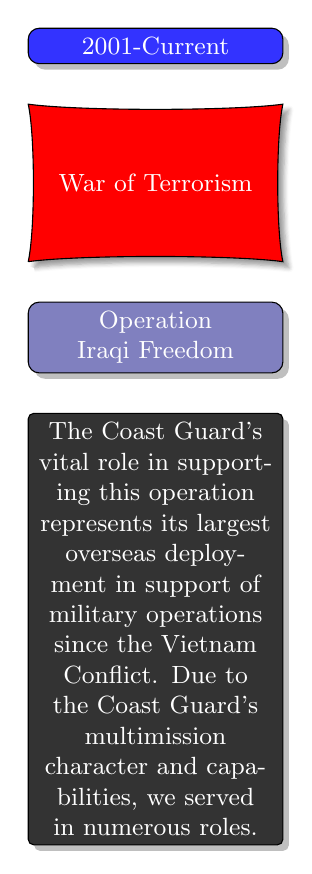
\begin{tikzpicture}[start chain=10 going below, start chain=11 going right, start chain=12 going right, node distance=5mm]
\node [box1, on chain=10]{2001-Current};
\node [b1, on chain=10]{War of Terrorism};
\node [box2, on chain=10]{Operation Iraqi Freedom};
\node [point, on chain=10]{The Coast Guard’s vital role in
supporting this operation represents its largest overseas deployment in
support of military operations since the Vietnam Conflict. Due to the
Coast Guard’s multimission character and capabilities, we served in
numerous roles.};

\end{tikzpicture}
\end{document}
